\makeheading{Lecture 19 | 2020-11-16}
\section{Prediction Error}
Sometimes a key application of a fitted model
is to do \underline{prediction} on new data
(and is more important than interpretability).

Previously, we saw model selection criteria
that are computed on fitted models
(AIC, BIC, Adjusted $ R^2 $) which assess
the explanatory
power of a model on the \emph{data used to fit the model}
(or \emph{train}).

While these criteria incorporate penalty terms to try
to prevent overfitting, they don't directly assess
how well a model would perform in predicting the response
on new data given predictors.

We mentioned metrics such as MSPE as measures of predictive
accuracy.

To assess accuracy in prediction, we need metrics for
measuring prediction error, e.g., evaluated
over $ m $ observations.

\begin{Definition}{Mean-squared Error (MSE)}{}
    If we have $ m $
    observations,
    \[ \text{MSE}=\frac{1}{m} \sum_{i=1}^{m} (y_i-\hat{y}_i)^2 \]
    where $ y_i $ is the actual value, $ \hat{y}_i $ is the
    predicted value (or equivalently, if we apply MSE on the fitted
    data, this would be the fitted value, $ \hat{\mu}_i $;
    if calculated on training data).
    Measured on the scale of $ \sigma^2 $.
\end{Definition}
\begin{Remark}{}{}
    MSE is equivalently called MSPE if applied on new data.
\end{Remark}
\begin{Definition}{Root-mean-squared Error (RMSE)}{}
    \[ \text{RSME}=\sqrt{\text{MSE}} \]
\end{Definition}
\begin{Remark}{}{}
    RMSE is measured on the scale of $ \sigma $.
\end{Remark}
\begin{Definition}{Mean Absolute Error (MAE)}{}
    \[ \text{MAE}=\frac{1}{m} \sum_{i=1}^{m} \abs{y_i-\hat{y}_i} \]
\end{Definition}
Ideally, we have lots of data, conceptualize having three parts.
\begin{table}[ht]
    \centering
    \begin{NiceTabular}{|>{\raggedright\arraybackslash}m{50mm}|m{50mm}|m{50mm}|}
        \toprule
        \multicolumn{1}{c}{Train $ (y_1,y_2,\ldots,y_n) $} & \multicolumn{1}{c}{Validation $ (y_{n+1},\ldots,y_{n+v}) $} & \multicolumn{1}{c}{Test $ (y_{n+v+1},\ldots,y_{n+v+t}) $} \\
        \midrule
        \textbullet~$ n $ observations.

        \textbullet~Fit models, as many as we want.
        &
        \textbullet~$ v $ observations.

        \textbullet~Estimate prediction error for each fitted model.
        &
        \textbullet~$ t $ observations.

        \textbullet~Used at the very end for final assessment of our selected model.\\
        \bottomrule
    \end{NiceTabular}
\end{table}

We have access to train and validation. Test data is from the future,
we won't have access to this until the data is released (say
the actual stock prices were released); that is, assume we don't get
to see this.

For example, using MSE as a metric, based on a fitted model we can
compute and compare:
\begin{table}[ht]
    \centering
    \begin{NiceTabular}{|c|c|c|}
        \toprule
        MSE Train & MSE Validation & MSE Test \\
        \midrule
        $ \frac{1}{n} \sum_{i=1}^{n} (y_i-\hat{y}_i)^2 $
        &
        $ \frac{1}{m} \sum_{i=n+1}^{n+v} (y_i-\hat{y_i})^2 $
        &
        $ \frac{1}{t} \sum_{i=n+v+1}^{n+v+t}(y_i-\hat{y}_i)^2 $
        \\
        \bottomrule
    \end{NiceTabular}
\end{table}

\begin{itemize}
    \item Observe ``MSE Train'' is equal to $ \displaystyle \frac{\SS{Res}}{n} $
          and our usual estimate of $ \hat{\sigma}^2 $
          is a scaled version of this quantity
          to compensate for the number of predictors. Specifically,
          $ \displaystyle  \hat{\sigma}^2=\frac{\SS{Res}}{n-p-1} $
          so it's unbiased.
    \item Consider ``MSE Validation'' as an \emph{estimate} of MSPE
          on new data.
    \item ``MSE Test'' is the actual test of prediction,
          we call this the \emph{actual} MSPE.\
\end{itemize}
\underline{Idea}: We hope that ``MSE Validation'' $ \approx $
``MSE Test'' since neither sets were used to fit the model.

\begin{minipage}{0.7\textwidth}
    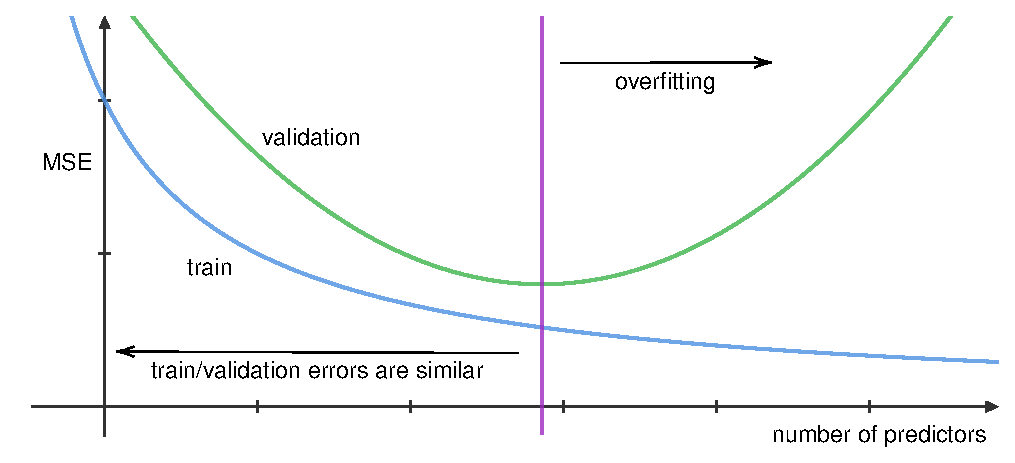
\includegraphics[width=\linewidth]{error.pdf}
\end{minipage}
\begin{minipage}{0.23\textwidth}
    \raggedright{}
    So, if we're using MSE/RMSE
    as a metric (as related to $ \hat{\sigma}^2 $ /$ \hat{\sigma} $)
    and the MSE/RMSE is significantly larger
    on validation compared to train,
    then we probably overfitted the model;
    that is, we can't expect the model
    to generalize well to new data.
\end{minipage}
\section{Cross-Validation}
How to use framework in practice:
\begin{itemize}
    \item Simplest: randomly divide available data
          between train/validation, say $ 80\% $/$ 20\% $ split.

          Weakness:
          \begin{enumerate}
              \item Don't use all data for training.
              \item Only get one estimate of prediction error.
          \end{enumerate}
    \item Better: Use cross-validation scheme (CV). How to
          do CV with $ K $ folds:
          \begin{figure}[!ht]
              \centering
              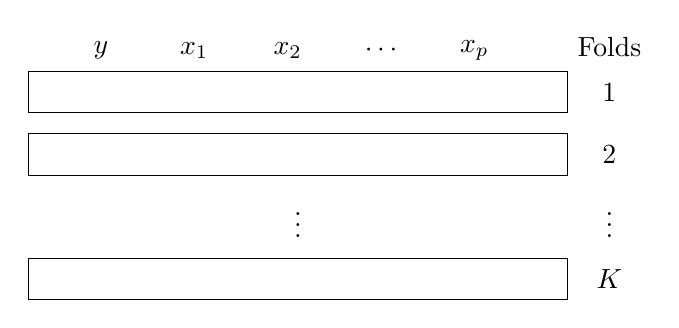
\begin{tikzpicture}[x=0.75pt,y=0.75pt,yscale=-1,xscale=1]
                  \draw (10,30) -- (270,30) -- (270,50) -- (10,50) -- cycle ;
                  \draw (10,60) -- (270,60) -- (270,80) -- (10,80) -- cycle ;
                  \draw (10,120) -- (270,120) -- (270,140) -- (10,140) -- cycle ;
                  \draw (140,100) node {$\vdots $};
                  \draw (290,40) node {$1$};
                  \draw (290,70) node {$2$};
                  \draw (290,100) node {$\vdots $};
                  \draw (290,130) node {$K$};

                  \draw (45,20) node {$y$};
                  \draw (90,20) node {$x_{1}$};
                  \draw (135,20) node {$x_{2}$};
                  \draw (180,20) node {$\cdots $};
                  \draw (225,20) node {$x_{p}$};
                  \draw (290,18) node {Folds};
              \end{tikzpicture}
          \end{figure}
          \begin{itemize}
              \item Divide available data for train and validation
                    into $ K $ roughly equally sized sets (folds),
                    usually randomly.
              \item For CV $ k $, use data in fold $ k $
                    as validation, and train on
                    the rest of data.
              \item Thus, to estimate the prediction error
                    \emph{for a given model}, we fit it $ K $ times, each
                    time treating the data in folds, $ 1,2,\ldots,K $
                    as validation.
                    Therefore, we get $ K $ estimates of prediction error
                    for that particular model.
              \item For example, using RMSE, we get
                    \[ \text{RMSE}_1,\text{RMSE}_2,\ldots,\text{RSME}_K \]
                    and can take the average
                    \[ \overline{\text{RSME}}=\frac{1}{K} \sum_{k=1}^{K}\text{RSME}_k \]
                    as an estimate for RMSPE on new data (test set).
          \end{itemize}
\end{itemize}
\subsection{R Demo}
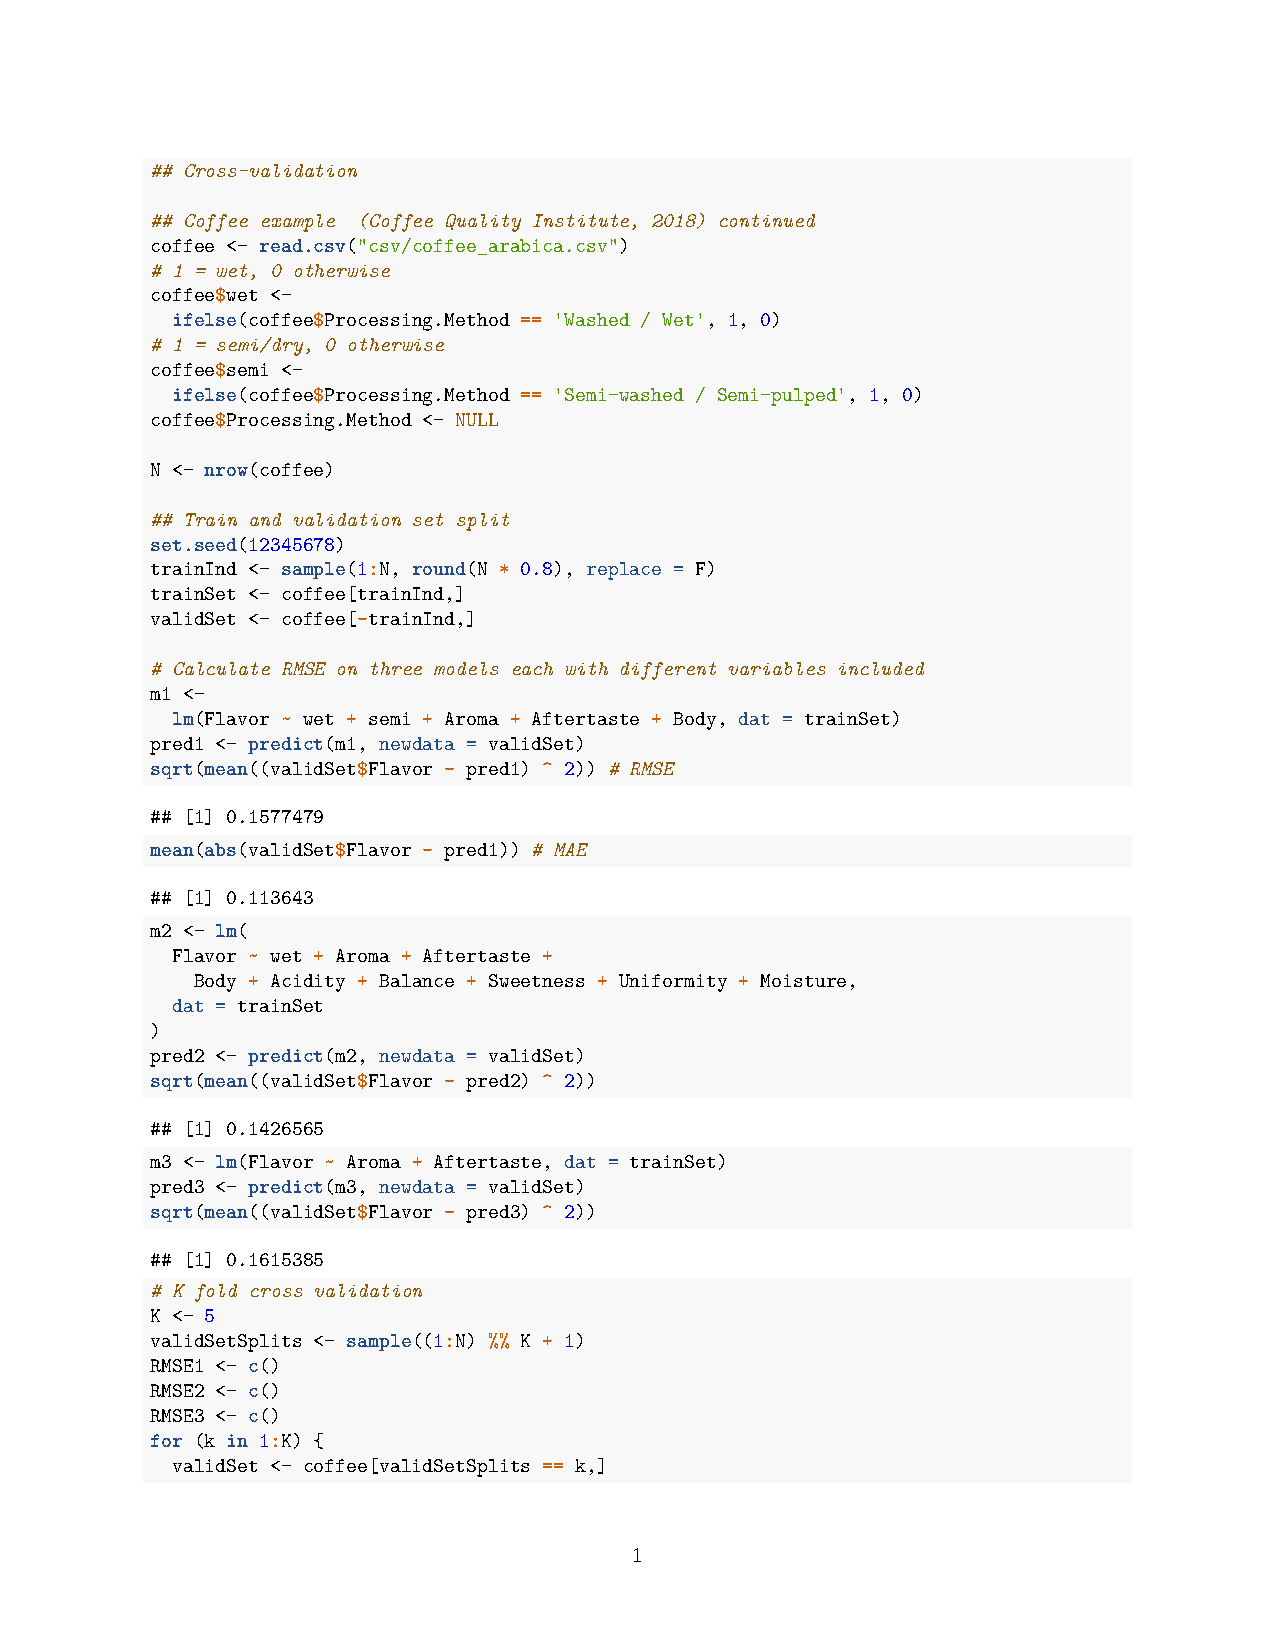
\includepdf[pages=-]{lec_19-demo.pdf}
